\documentclass[draftspec]{sbmlpkgspec}
\usepackage{tabularx}

\begin{document}

\packageTitle{The Distributions Package\\for SBML Level 3}
\packageVersion{Version 0.7 (Draft)}
\packageVersionDate{6 August, 2012}
%\packageGeneralURL{http://sbml.org/Community/Wiki/SBML_Level_3_Proposals/Distributions_and_Ranges}
%\packageThisVersionURL{}

\author{%
  \begin{tabular}{c>{\hspace{20pt}}c}
    \multicolumn{2}{c}{\Large\bf{Authors}}\\\\
    Stuart L Moodie&Darren Wilkinson\\
    \mailto{moodie@ebi.ac.uk}&\mailto{darren.wilkinson@ncl.ac.uk}\\
    EMBL-EBI& University of Newcastle\\
    Hinxton, UK& Newcastle, UK\\
   \\
    Nicolas Le Nov\`{e}re\\
    \mailto{lenov@ebi.ac.uk}\\
    EMBL-EBI\\
     Hinxton, UK\\\\
    \multicolumn{2}{c}{\Large\bf{Contributors}}\\\\
     \multicolumn{2}{c}{ Colin Gillespie}\\
     \multicolumn{2}{c}{\mailto{c.gillespie@ncl.ac.uk}}\\
     \multicolumn{2}{c}{University of Newcastle}\\
     \multicolumn{2}{c}{ Newcastle, UK}\\
\end{tabular}
}

\notice{Disclaimer: This is a working draft of the SBML Level 3
  ``distib'' package proposal. It is not a normative document.  Please
  send comments and other feedback to the mailing list:
  \mailto{sbml-distrib@lists.sourceforge.net.}}

\maketitlepage
\maketableofcontents

\newcommand\arrays{Arrays and Sets\xspace}
\newcommand\arraysshort{arrays\xspace}
\newcommand\distribshort{distrib\xspace}
\newcommand\distrib{Distributions\xspace}
\newcommand\uncertml{UncertML\xspace}
\newcommand\numl{NuML\xspace}
\newcommand\unidistrib{\abstractclass{IUncertainty}\xspace}
\newcommand\mlambda{\class{Lambda}\xspace}
\newcommand\mmath{\class{Math}\xspace}
\newcommand\Distribution{\defRef{Distribution}{sec:distribution}}
\newcommand{\mathml}{MathML\xspace}

\reversemarginpar  % Want "\watchout" to be put on the left, not the right.
\newcommand{\watchout}{\marginpar{\hspace*{34pt}\raisebox{-0.5ex}{\Large\ding{43}}}}
\newcommand{\contraversial}{\marginpar{\hspace*{34pt}\raisebox{-0.5ex}{\Large?}}}

\section*{Revision History}

\begin{edtable}{tabularx}{\linewidth}{c c c X }\toprule
\textbf{Version} & \textbf{Date} & \textbf{Author} & \textbf{Comments} \\ \midrule
0.1 (Draft) & 15 Oct 2011 & Stuart Moodie & First draft \\ \midrule
0.2 (Draft) & 16 Oct 2011 & Stuart Moodie & Added introductory text
and background info. Other minor changes etc. \\ \midrule
0.3 (Draft) & 16 Oct 2011 & Stuart Moodie & Filled empty invocation
semantics section.\\ \midrule
0.4 (Draft) & 4 Jan 2012 & Stuart Moodie & Incorporated comments from
NlN, MS and SK. Some minor revisions and corrections.\\  \midrule
0.5 (Draft) & 6 Jan 2012 & Stuart Moodie & Incorporated addition
comments on aim of package from NlN.\\ \midrule
0.6 (Draft) & 19 Jul 2012 & Stuart Moodie & Incorporated revisions
discussed and agreed at HARMONY 2012.\\ 
0.7 (Draft) & 6 Aug 2012 & Stuart Moodie & Incorporated review
comments from Maciej Swat and Sarah Keating.\\ 
\bottomrule
\end{edtable}

\section{Introduction and motivation}

\subsection{What is it?}

The \distrib package (also affectionately known as \distribshort for
short) provides an extension to SBML Level 3 that enables it to encode
models that sample values from statistical distributions. Applications
of the package include for instance descriptions population based
models: an important subset of which are
pharmacokinetic/pharmacodynamic (PK/PD) models\footnote{for more
  information see: \url{http://www.pharmpk.com/}.}, which are used to
model the action of drugs.

Note that originally the package was called Distributions and Ranges,
but Ranges are no longer in the scope of this hence the name change.

\subsection{Scope}

The \distrib package adds support to SBML for sampling from a
probability distribution in parts of an SBML model that are
\textbf{not} continuously evaluated. in particular the following are
in scope:

\begin{itemize}
\item Sampling from a continuous distribution.
\item Sampling from a discrete distribution.
\item Sampling from user-defined probability density function.
\item Sampling from user-defined discrete probability density.
\end{itemize}

At one point the following were considered for inclusion in this
package but are now \textbf{out of scope}:

\begin{itemize}
\item Stochastic differential equations.
\item Cumulative distribution functions.
\item Description of the uncertainty of a model parameter: for
  example, standard deviation, standard error and similar descriptive
  statistics.\footnote{It is proposed that this be provided
    descriptive statistics in a separate package.}
\end{itemize}

\subsection{This Document}

The authors' expectation is that this is close to a final draft of the
proposal with only a limited number of issues to be resolved. In its
current state this document aims to establish a consensus about what
has been agreed and what work remains to be carried out to complete
the definition of this package.

This proposal is a working document and once finalised will be the
first step towards the formal adoption of the \distribshort as a
package in SBML Level 3. After this two implementations based on this
proposal are required and then a vote on its adoption by the SBML
community. The proposal will then provide the basis for a future
package specification document. More details of the SBML package
adoption process can be found at:
\url{http://sbml.org/Documents/SBML_Development_Process}.

Please also note that in this draft of the proposal a list of the
exact probability distributions to be supported has not been
included. This is because at present it is envisaged that
\distribshort will refer to an external definition of probability
distributions (see sections \ref{sec:externaldistdef} and
\ref{sec:unresolved}).

\subsection{Conventions used in this document}

As we are early in the package proposal process there will be some
parts of this proposal where there is no clear consensus on the
correct solution or only recent agreement or agreement by a group
which may not be representative of the SBML community as a
whole. These cases are indicated by the \contraversial question mark
in the left margin (illustrated). The reader should pay particular
attention to these points and ideally provide feedback, especially if
they disagree with what is proposed. Similarly there will be points
--- especially as the proposal is consolidated --- which are agreed,
but which the reader should take note of and perhaps read again. These
points \watchout are emphasised by the hand pointer in the left margin
(illustrated),

\section{Background}

\subsection{Problems with current SBML approaches}

SBML Level 3 Core has no direct support for providing random values
within a model. Currently there is no workaround and this makes it
impossible to describe models that use probability distributions.

\subsection{Past work on this problem or similar topics}

\subsubsection{The Newcastle Proposal}
\label{sec:newcastle proposal}

In 2005 there was a proposal from Colin Gillespie and others
\footnote{\url{http://sbml.org/Community/Wiki/SBML_Level_3_Proposals/Distributions_and_Ranges}}
to introduce support for probability distributions in the SBML core specification. This
was based on their need to use such distributions to represent the
models they were creating as part of the BASIS project
\url{http://www.basis.ncl.ac.uk}).

They proposed that distributions could be referred to in SBML using
the \class{csymbol} element in the \mathml subset used by
the SBML Core specification. An example is below:

\begin{example}
<xmlns=''http://www.w3.org/1998/Math/MathML''>
  <apply>
    <csymbol encoding=''text''
        definitionURL=''http://www.sbml.org/sbml/symbols/uniformRandom''>
      uniformRandom
    </csymbol>
    <ci>mu</ci>
    <ci>sigma</ci>
  </apply>
</math>
\end{example}

This required that a library of definitions be maintained as part of
the SBML standard and in their proposal they defined an initial small
set of commonly used distributions. The proposal was never
implemented.

\subsubsection{Seattle 2010}

The ``distrib'' package was discussed at the Seattle SBML Hackathon%
\footnote{\url{http://sbml.org/Events/Hackathons/The_2010_SBML-BioModels.net_Hackathon}}. There
one of the authors (DW) presented an overview of the problem%
\footnote{Slides:
 \url{http://sbml.org/images/3/3b/Djw-sbml-hackathon-2010-05-04.pdf}}%
\footnote{Audio:
  \url{http://sbml.org/images/6/67/Wilkinson-distributions-2010-05-04.mov}},
building on the old proposal from the Newcastle group
 (see above: \ref{sec:newcastle proposal}).
There was broad support at the meeting for development of such a
package, and for the proposed feature set. Discussion following the
presentation led to a consensus on the following points:

\begin{itemize}
\item There is an urgent need for such a package.
\item It is important to make a distinction between a description of
  uncertainty regarding a model parameter and the mechanistic process
  of selecting a random number from a probability distribution, for
  applications such as parameter scans and experimental design
\item It is probably worth including the definition of PMFs, PDFs and CDFs in the package
\item It is worth including the definition of random distributions using particle representations within such a package, though some work
 still needs to be done on the precise representation
\item It could be worth exploring the use of xinclude to point at particle
representations held in a separate file
\item Random numbers must not be used in rate laws or anywhere else that
 is continuously evaluated, as then simulation behaviour is not
 defined
\item Although there is a need for a package for describing extrinsic
 noise via stochastic differential equations in SBML, such mechanisms
 should not be included in this package due to the considerable
 implications for simulator developers
\item We probably don't want to layer on top of \uncertml
 (www.uncertml.org), as this spec is fairly heavy-weight, and
 somewhat tangential to our requirements
\item A random number seed is not part of a model and should not be
 included in the package
\item The definition of truncated distributions and the specification of
 hard upper and lower bounds on random quantities should be
 considered.
\end{itemize}

It was suggested that new constructs should be introduced into SBML by
the package embedded as user-defined functions using the following
syntax:

\begin{example}
<listOfFunctionDefinitions>
  <functionDefinition id="myNormRand">
    <distrib:####>
      #### distrib binding information here ####
    </distrib:####>
    <math>
      <lambda>
        <bvar>
          <ci>mu</ci>
          <ci>sigma</ci>
        </bvar>
        <ci>mu</ci>
      </lambda>
    </math>
  </functionDefinition>
</listOfFunctionDefinitions>
\end{example}

which allows the use of a "default value" by simulators which do not
understand the package (but simulators which do will ignore the <math>
element). The package would nevertheless be "required", as it will not
be simulated correctly by software which does not understand the
package.

Informal discussions following the break-out covered topics such as
how to work with vector random quantities in the absence of the vector
element in the MathML subset used by SBML, and the care that must be
taken with the semantics of random variables and the need to both a)
reference multiple independent random quantities at a given time and
b) make multiple references to the same random quantity at a given
time.

\subsubsection{Hinxton 2011}

Detailed discussion was continued at the Statistical Models Workshop
in Hinxton in June 2011%
\footnote{\url{http://sbml.org/Events/Other_Events/statistical_models_workshop_2011}}. There
those interested in representing Statistical Models in SBML came
together to work out the details of how this package would work in
detail. Dan Cornford from the \uncertml
project\footnote{\url{http://www.uncertml.org/}} attended the meeting
and described how that resource could be used to describe uncertainty
and in particular probability distributions. Perhaps the most
significant decision at this meeting was to adopt the \uncertml
resource as a controlled vocabulary that is referenced by the \distrib package.

Much of the detail and the examples in this proposal are based on
the work of this workshop and so its outcomes are essentially
presented below. However, at the end of the meeting there remained a
number of unresolved issues that are still unresolved in this
proposal. See section \vref{sec:unresolved} for more details.


\subsubsection{HARMONY 2012: Maastricht}

Two sessions were dedicated to discussion of \distrib at HARMONY based
around the proposals described in version 0.5 of this document. In
addition there was discussion about the \arrays proposal which was
very helpful in solving the problem of multivariate distributions in
\distrib. The following were the agreed outcomes of the meeting:

\begin{itemize}
\item The original proposal included UncertML markup directly in the
  function definition. This proved unwieldy and confusing and has been
  replaced by a more elegant solution that eliminates the UncertML
  markup and integrates well with the fallback function (see details
  below).
\item Multivariate distributions can be supported using the \arrays
  package to define a covariance matrix.
\item User defined continuous distributions would define a PDF in
  \mathml.
\item Usage semantics were clarified so that invokation of a function
  definition implied a value was sampled from the specified
  distribution.
\item It was agreed from which sections of an SBML model a
  distribution could be invoked.
\item Statistical descriptors of variables (for
  example mean and standard deviation) would be separated from
  \distrib and either provided in a new package or in a later version
  of SBML L3 core.
\end{itemize}

\section{Proposed syntax and semantics}

\subsection{Colour Conventions}

Throughout this document, in all UML diagrams, classes that exists in
SBML Level 3 core or another existing standard are displayed in
black. If those elements are extended in this proposal, those
extensions are displayed in green. Classes that are new to this
proposal are shown in blue.

\subsection{Defining Distributions}

The \distrib package has a very simple purpose. It defines a
statistical distribution, range or statistic from which you can obtain
a value that is used in other parts of an SBML model. The distribution
is defined using \uncertml, which is a resource that defines
probabilistic uncertainties~\cite{uncertml}, or explicitly using
MathML~\cite{mathml2}.

SBML Core is extended at the \FunctionDefinition class as can be seen
in the UML representation in figure \vref{fig:umlmodel}. The extended
\FunctionDefinition can optionally contain a single instance of a new
class \class{Distribution} that is part of the distrib package. The \class{Distribution} class can
then either refer to an element in UncertML using or alternatively a
\class{Distribution} can contain a \mmath class that is used to define the
distribution explicitly.

\begin{figure}[htb]
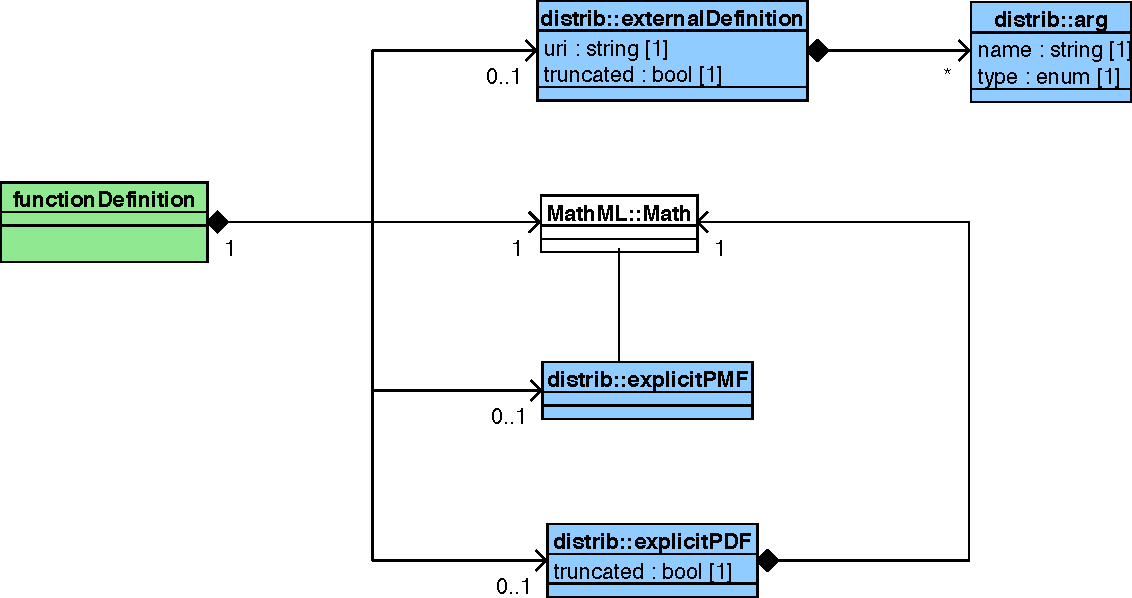
\includegraphics[width=1.0\linewidth]{DistribUMLModel.pdf}
\caption{UML class diagram for the \distrib package. This diagram describes the
  classes involved and not instances of those classes. Note the UML packages
  indicate that the classes belong to different namespaces. The
  namespace of the SBML Core is not shown.}
\label{fig:umlmodel}
\end{figure}

\subsection{Extension Handling}

The \distrib package is defined as a required package, which means
that an SBML model that uses that extension will not be correctly
defined unless the features of the extension are used and interpreted
correctly by supporting software.

\subsection{FunctionDefinition Extension}

As outlined above the \FunctionDefinition is extended to include the attributes defined below.

\paragraph{\token{function}}

This provides the external definition of the distribution to be
invoked. The value of the attribute should be a URI that
uniquely identifies a definition from an external resource. The exact
nature of this URI and the external resource to use is discussed below
(section \ref{sec:extlDefnDistn}). The attribute is optional.

\paragraph{\token{explicit}}

This attribute indicates that a user-defined (or explicit) continuous
distribution will be defined. If it has a value of \texttt{true} then
the \mathml expression in the body of the function definition should
define a probability definition function. In this case this also
serves as the fallback function. Note that a user define discrete
distribution is defined in a different way (see section
\ref{sec:userDefinedDiscrete}).

\subsubsection{Usage Rules}

The \token{function} cannot have a value (i.e.\xspace it must be
\texttt{null}) when the \token{explicit} attribute has a value of
\texttt{true}.

\subsection{Using the \distribshort package}

The distribution defined by a \FunctionDefinition instance can be
used by instances of the following SBML classes:

\begin{itemize}
  \item InitialAssignment
  \item EventAssignments
  \item Delays
  \item Priorities
\end{itemize}

An invocation of a distribution behaves like any other function call
in SMBL and the function is executed. For a statistical distribution
this means that one or more values are sampled from the distribution
each time the function definition is invoked.

\subsection{Permitted Types}

The \distrib package will support arrays and matrices via the \arrays
package. This means that paramaters passed to a function definition
can be arrays, matrices or scalar values and that a functions return
type can be either a scalar or the above non-scalar types. Type
consistency and conversion behaviour between scalar and non-scalar
types is defined by the \arrays package.

\subsection{External Definition of Distributions}
\label{sec:extlDefnDistn}
\label{sec:externaldistdef}

The external definition is a URI that should refer to a standardised
dictionary of distributions. It should unambiguously define the
following:

\begin{itemize}
\item A globally unique URI by which to refer to it.
\item A meaningful name
\item The parameter arguments used by the function, including for each
 argument: its name and type (scalar or non-scalar). Note that all
 arguments are mandatory.
\item The value and its type returned by the function.
\item A detailed mathematics description of the statistical distribution being
  sampled from.
\end{itemize}

The exact specification of the URI is undefined at the moment and will
be finalised once the source of the external definition has been
agreed. See unresolved issues below (section
\ref{sec:unresolved}).


\subsection{Equivalence with Fallback Function}

The \mathml definition contained in the function definition is not
used if \distribshort is supported and the \token{explicit} attribute
is \texttt{false}. However, in order to ensure the SBML model is still
valid when \distribshort is not supported the fallback function must
be present and it should conform to the following rules:

\begin{itemize}
\item Match the number of arguments in the external function
  definition.
\item Each argument should match the type of the equivalent argument
  in the external function.
\item Have the same return type as the external function.
\end{itemize}

Clearly these rules can only be enforced when \distrib is supported.

\section{Package dependencies}

This package is dependent on the \arrays package to provide array and
matrix structures. It is also dependent on \mathml \cite{mathml2} to
define distributions explicitly. It uses the the subset of \mathml set
out in the SMBL Level 3 Core Specification
\cite{l3v1c}.

\section{Use-cases and examples}

\subsubsection{Sampling from a distribution: PK/PD Model}

This is a very straightforward use of an externally defined
distribution. The key point to note is that a value is sampled from
the distribution and assigned to a variable when it is invoked. In the
initialAssignments element in this example. Later use of the variable
does not result in re-sampling from the distribution. This is
consistent with current SBML semantics.

\exampleFile{examples/pkpd.xml}

\subsection{Truncated distribution}
\label{sec: truncated-eg}

To encode a truncated distribution we rely on external
definitions. Clearly it would be cumbersome if every distribution and
multivariate distribution required a truncated equivalent definition,
but at present this is what is required\contraversial. Perhaps this
problem could be solved if optional function arguments were permitted,
but this cases problems with the fallback function (see section \ref{sec:unresolved}).

\exampleFile{examples/truncated_distn.xml}

\subsection{Multivariate distribution}

In this example two correlated parameters are sampled from a
multivariate distribution. The correlation is defined using a
covariance matrix and the sampled values are returned as a vector of 2
values, which are then assigned to the individual parameters. This
example relies heavily on the \arraysshort package, which will be a
dependency of the \distribshort package.

\exampleFile{examples/mutivariate_example.xml}

\subsection{User-defined continuous distribution }

In this example an additional construct is used to indicate:
\begin{itemize}
\item that the \mathml within the function definition defines a PDF and so is not a
fallback.
\item that when invoked a value should be sampled from this PDF.
\end{itemize}

\exampleFile{examples/user-defined.xml}


\subsection{User-defined discrete distribution}
\label{sec:userDefinedDiscrete}

In this example we don't use any special distrib features, by invoke
an externally defined function that constructs a PMF from a matrix of
values and their associated probabilities. The example is not
biologically meaningful, but illustrates that the matrix contains the
values and probabilities possible when throwing two dice. These values
are encoded in a matrix, which is passed as a parameter in a function,
however, it may be that this information is defined using
\numl\contraversial or by referring to an external file.

There has been very little discussion\contraversial{} about how to treat user-defined
PMFs so this example should be regarded as a starting point for
discussion rather than a final proposal.

\exampleFile{examples/user-defined-pmf.xml}

\section{Prototype implementations}

None as yet.

\section{Unresolved issues}
\label{sec:unresolved}

\begin{description}
\item[what external distrib definition?] A key decision is what form the
  external definition of the distributions will take. In particular
  should we use \uncertml, a definition based on a snapshot of
  \uncertml, another controlled vocabulary yet to be identified or do
  we create our own?
\item[Optional function arguments] It would be useful to provide
  optional arguments to functions, which at the moment is not
  possible. This would provide a convenient method for defining
  truncated distributions: all distributions could have an optional
  min and max argument that defaults to $-\inf$ and $+\inf$
  respectively, but when set to a value it explicitly defines a
  truncated function.
\end{description}

\section{Acknowledgements}

Much of the initial concrete work leading to this proposal document
was carried out at the Statistical Models Workshop in Hinxton this
year (2011). A list of participants and recordings of the discussion
is available from
\url{http://sbml.org/Events/Other_Events/statistical_models_workshop_2011}.
The authors would also like to thank the participants of the
\distribshort sessions during HARMONY 2012 for their excellent
contributions in helping revising this proposal into something a lot
closer to the finished version.

The authors would like to thank Sarah Keating and Maciej Swat for
useful discussions; and Mike Hucka for \LaTeX{} advice and his
beautiful template upon which this document is based.

%\appendix
%\section{Appendix}

\bibliography{sbml-level-3-distrib-package-proposal}


\end{document}

